% Options for packages loaded elsewhere
\PassOptionsToPackage{unicode}{hyperref}
\PassOptionsToPackage{hyphens}{url}
\documentclass[]{article}
\usepackage{xcolor}
\usepackage{amsmath,amssymb}
\setcounter{secnumdepth}{-\maxdimen} % remove section numbering
\usepackage{iftex}
\ifPDFTeX
  \usepackage[T1]{fontenc}
  \usepackage[utf8]{inputenc}
  \usepackage{textcomp} % provide euro and other symbols
\else % if luatex or xetex
  \usepackage{unicode-math} % this also loads fontspec
  \defaultfontfeatures{Scale=MatchLowercase}
  \defaultfontfeatures[\rmfamily]{Ligatures=TeX,Scale=1}
\fi
\usepackage{lmodern}
\ifPDFTeX\else
  % xetex/luatex font selection
\fi
% Use upquote if available, for straight quotes in verbatim environments
\IfFileExists{upquote.sty}{\usepackage{upquote}}{}
\IfFileExists{microtype.sty}{% use microtype if available
  \usepackage[]{microtype}
  \UseMicrotypeSet[protrusion]{basicmath} % disable protrusion for tt fonts
}{}
\makeatletter
\@ifundefined{KOMAClassName}{% if non-KOMA class
  \IfFileExists{parskip.sty}{%
    \usepackage{parskip}
  }{% else
    \setlength{\parindent}{0pt}
    \setlength{\parskip}{6pt plus 2pt minus 1pt}}
}{% if KOMA class
  \KOMAoptions{parskip=half}}
\makeatother
\usepackage{longtable,booktabs,array}
\newcounter{none} % for unnumbered tables
\usepackage{calc} % for calculating minipage widths
% Correct order of tables after \paragraph or \subparagraph
\usepackage{etoolbox}
\makeatletter
\patchcmd\longtable{\par}{\if@noskipsec\mbox{}\fi\par}{}{}
\makeatother
% Allow footnotes in longtable head/foot
\IfFileExists{footnotehyper.sty}{\usepackage{footnotehyper}}{\usepackage{footnote}}
\makesavenoteenv{longtable}
\usepackage{graphicx}
\makeatletter
\newsavebox\pandoc@box
\newcommand*\pandocbounded[1]{% scales image to fit in text height/width
  \sbox\pandoc@box{#1}%
  \Gscale@div\@tempa{\textheight}{\dimexpr\ht\pandoc@box+\dp\pandoc@box\relax}%
  \Gscale@div\@tempb{\linewidth}{\wd\pandoc@box}%
  \ifdim\@tempb\p@<\@tempa\p@\let\@tempa\@tempb\fi% select the smaller of both
  \ifdim\@tempa\p@<\p@\scalebox{\@tempa}{\usebox\pandoc@box}%
  \else\usebox{\pandoc@box}%
  \fi%
}
% Set default figure placement to htbp
\def\fps@figure{htbp}
\makeatother
\usepackage{svg}
\setlength{\emergencystretch}{3em} % prevent overfull lines
\providecommand{\tightlist}{%
  \setlength{\itemsep}{0pt}\setlength{\parskip}{0pt}}
\usepackage{bookmark}
\IfFileExists{xurl.sty}{\usepackage{xurl}}{} % add URL line breaks if available
\urlstyle{same}
\hypersetup{
  hidelinks,
  pdfcreator={LaTeX via pandoc}}

\author{}
\date{}

\begin{document}

\textbf{Adversarial Sponge Attack: Exploiting Resource Depletion Vulnerabilities on Edge Servers via Spatial Optimization}\\
\emph{Adversarial Sponge Attack: Visual Denial-of-Service on Edge Server}

\textbf{Tuan Anh Pham,}\\
Ho Chi Minh City University of Technology (HUTECH), Vietnam.\\
Email: anh25807700004@hutech.edu.vn

\textbf{Quoc Bao Mai,}\\
Ho Chi Minh City University of Technology (HUTECH), Vietnam.\\
Email: bao2580770008@hutech.edu.vn

\textbf{ABSTRACT}

The deployment of Edge Servers in security surveillance brings significant benefits but simultaneously exposes critical vulnerabilities in resource management. While current Adversarial Attack research predominantly focuses on Misclassification, this paper proposes a novel threat vector directly targeting system Availability: Resource Depletion Attacks via Sponge Patches. The core contribution of this research is a Gray-box optimization framework, assuming the attacker has access only to the neural network's internal telemetry prior to the post-processing filter. The proposed method integrates Saliency Maps for active spatial localization of sensitive regions and Genetic Algorithms to accelerate convergence. The generated Sponge Patch forces CNNs to predict thousands of phantom bounding boxes, directly exploiting the \(\mathcal{O}\left( N^{2} \right)\) computational bottleneck of the Non-Maximum Suppression (NMS) algorithm. Experiments via Digital Injection into real-time IP Camera streams demonstrate that the attack pushes average CPU load from 52--64\% up to 67--78\% (peaking at 100\% as recorded in Figure 5), consumes 4.8GB of RAM, and severely degrades FPS to 5-11. Preliminary Physical Testing confirms the feasibility of the method when deployed through optical lenses, achieving a 60\% CPU load. This research substantiates the imminent risk of Visual DoS, posing an urgent requirement for hardware-resilient defense designs. Source code is available at:
https://github.com/reikageisme/Physical-Visual-DoS-EdgeAI

\emph{\textbf{Keywords} :} \emph{Gray-box Adversarial Attack, Visual DoS, Sponge Patch, Edge Server, Non-Maximum Suppression (NMS)}

\textbf{1. INTRODUCTION}

\textbf{1.1. Problem Statement}

Deep Learning models, particularly Convolutional Neural Networks (CNNs), play a fundamental role in computer vision systems such as security surveillance cameras and autonomous vehicles. The architectural shift from cloud computing to Edge computing (Edge-AI) offers substantial advantages in terms of low latency and data privacy. However, this trend concurrently presents a practical infrastructure challenge: current surveillance systems frequently utilize outdated hardware configurations as Legacy On-Premise Edge Servers. These legacy x86 hardware systems entirely lack Graphics Processing Units (GPUs) or dedicated AI acceleration cores, resulting in exceptionally strict limitations on computational resources (CPU, RAM) and thermal dissipation capabilities when tasked with real-time inference.

Recently, the concept of Sponge Attacks has emerged to deplete AI energy resources {[}6, 8, 9{]}, but they are mostly confined to White-box and Digital Attack scenarios. The pressing challenge is: Can an attacker deplete the hardware resources of an Edge-AI system through a \textbf{Gray-box} scenario---where only partial internal telemetry is exploited without source code intervention?

\textbf{1.2. Research Objectives}

This research aims to construct an entirely novel Visual DoS adversarial attack pipeline, directly targeting the resource vulnerabilities of Legacy On-Premise Edge Servers by bottlenecking the Non-Maximum Suppression (NMS) post-processing algorithm \textbf{{[}11, 12{]}}. Specific objectives include:

\begin{enumerate}
\def\labelenumi{\arabic{enumi}.}
\item
  \textbf{Developing a Gray-box optimization mechanism:} Utilizing gradient-free Genetic Algorithms {[}17{]} combined with the extraction of raw anchors prior to the post-processing filter to generate the Sponge Patch.
\item
  \textbf{Optimizing the attack space:} Applying Saliency Maps {[}16{]} to determine the most sensitive coordinates on the frame, narrowing the search space and increasing convergence speed.
\item
  \textbf{Ensuring robustness:} Integrating Expectation Over Transformation (EOT) techniques to maintain destructive capability against visual perturbations caused by imaging devices.
\item
  \textbf{Verifying practical threat levels:} Deploying experiments on legacy server hardware (Edge Server - Intel Core i5) across two scenarios: Digital Injection and Preliminary Physical Testing, to accurately measure and quantify Visual DoS capabilities.
\end{enumerate}

\begin{quote}
\textbf{1.3. Research Contributions}
\end{quote}

This research does not aim to compare the load-bearing capacity of hardware, but rather focuses on proposing an attack sample generation method with high accuracy, fast convergence, and low computational resource footprint. Core contributions include:

\textbf{a. Baseline Foundation:}\\
The research builds upon the theoretical foundation of Adversarial Patches proposed by Brown et al. \hyperref[TL1]{\textbf{{[}1{]}}}, combined with the Expectation Over Transformation (EOT) technique by Athalye et al. \hyperref[TL2]{\textbf{{[}2{]}}} to ensure the viability of the adversarial sample in the real world.

\textbf{b. Novel Contributions:}\\
Unlike previous studies that only targeted classifier deception, this project contributes a groundbreaking Visual DoS attack sample generation method, particularly optimized for constrained research resource conditions:

\begin{enumerate}
\def\labelenumi{\arabic{enumi}.}
\item
  \textbf{Proposing a Saliency-Guided Genetic Algorithm optimization framework:} Overcoming the drawbacks of blind searching, integrating Saliency Maps helps the algorithm actively locate sensitive spatial regions. This enables the system to achieve fast convergence and generate high-accuracy attack samples without relying on expensive training server infrastructure.
\item
  \textbf{Proposing a Gray-box Fitness Function:} Focusing directly on maximizing neuron activation energy prior to NMS instead of optimizing the Cross-Entropy loss function like traditional White-box attacks. The assumed attacker only collects the quantity and confidence scores of internal bounding boxes instead of accessing the entire model weights.
\item
  \textbf{Presenting and proving mathematical vulnerabilities:} Clarifying the bottleneck mechanism with a complexity of \(\mathcal{O}\left( N^{2} \right)\ \) of the NMS post-processing algorithm when faced with dense noise data generated by the Sponge Patch.
\item
  \textbf{Providing empirical evidence and Domain Gap analysis:} Presenting quantitative data on hardware bottleneck capabilities in the Digital Injection scenario, while offering an objective preliminary assessment of damage degradation in physical environments (Physical Testing).
\end{enumerate}

\textbf{1.4. Research Questions}

To address the Visual DoS attack problem on Edge-AI systems, this research focuses on answering three core questions:

\textbf{RQ1 (Regarding vulnerability feasibility):} Is the Non-Maximum Suppression (NMS) post-processing algorithm with a complexity of \(\mathcal{O}\left( N^{2} \right)\) truly a "weak point" causing computational resource depletion (CPU, RAM) on legacy Edge Servers when confronted with dense noisy data?

\textbf{RQ2 (Regarding optimization methodology):} How can an effective Fitness Function be designed for a Genetic Algorithm combined with a Saliency Map to optimize the Sponge Patch in a \textbf{Gray-box} scenario, where the attacker only has access to the internal prediction parameter stream?

\textbf{RQ3 (Regarding physical robustness):} How does the Domain Gap between the digital environment and physical reality affect the destructive power of the attack when deployed through IP camera lenses and subjected to variations in lighting and viewing angles?

\textbf{2. RELATED WORKS}

Between 2022 and the present, the field of Adversarial Attacks on computer vision systems has witnessed a profound paradigm shift. Instead of solely generating perturbations in the digital space, modern research focuses on feasibility in physical environments and targets state-of-the-art neural network architectures. Based on their disruptive objectives, recent works are primarily divided into two main branches: Misclassification Attacks and Resource-Depletion Attacks.

\textbf{2.1. Digital Adversarial Attacks}

Since 2022, Adversarial Patch generation methods have surpassed the limitations of static 2D printed patterns. Several studies, typically the AdvReal framework by Huang et al. \textbf{{[}15{]}}, have optimized patches to deceive recognition systems in both 2D and 3D environments under severe lighting and viewing angle conditions. Although achieving high Robustness in practice, the core limitation of this entire research branch is that they solely target data Integrity. That is, the patch only causes the AI to misclassify, while the hardware system and FPS continue to function entirely normally.

\textbf{2.2. Physical Adversarial Attacks}

To disrupt system Availability, the concept of Sponge Examples was introduced by Shumailov et al. \textbf{{[}6{]}} as a novel threat vector. Instead of degrading accuracy, attackers fabricate specific input data to force neural networks into executing the densest computational sequences, drastically spiking inference latency and energy consumption.

Particularly in object detection tasks, the \emph{Phantom Sponges} study by Shapira et al. \textbf{{[}11{]}} demonstrated that the Non-Maximum Suppression (NMS) post-processing algorithm is the actual hardware "bottleneck". By injecting noise, they create "phantom" objects that NMS is forced to process with an \(\mathcal{O}\left( N^{2} \right)\) complexity, significantly increasing the processing time per frame. However, current NMS attack methods (like Phantom Sponges) reveal a fatal flaw: They are confined to the Digital Domain by injecting noise directly into Universal Adversarial Perturbations (UAP), which cannot be printed and deployed in a physical form.

\textbf{Research Gap:}

There is a noticeable disconnect between the two aforementioned research streams: Physical attacks cannot deplete resources, while resource-depletion attacks cannot be deployed in restricted access modes (Gray-box/Black-box). The Visual DoS attack scenario that meets all three criteria: \textbf{(1) Real-time noise injection capability and preliminary physical feasibility, (2) Operation within a Gray-box scenario, and (3) Efficacy on resource-constrained Edge-AI devices, remains an comprehensively unsolved problem}.

\textbf{2.3. Our Approach}

To bridge the gap outlined above, our research integrates the power of Evolutionary Algorithms and physical simulation techniques to create a groundbreaking Visual DoS attack:

\begin{enumerate}
\def\labelenumi{\arabic{enumi}.}
\item
  \textbf{Saliency-Guided Gray-box Optimization:} Overcoming the disadvantage of White-box methods (which require full access to weights and gradients), the proposed system utilizes a Genetic Algorithm in a Gray-box scenario. The hypothetical attacker only needs to collect internal telemetry parameters (raw anchors and confidence scores) from the model as feedback signals. Crucially, the integration of Saliency Maps {[}16{]} enables the algorithm to actively locate the "vital point" on the frame to evolve the patch, helping to maximize damage without increasing the physical dimensions of the adversarial sample.
\item
  \textbf{NMS Bottleneck Exploitation:} Proposing a completely novel Fitness Function. The patch is trained to force the CNN to output thousands of phantom bounding boxes simultaneously. This massive volume of garbage data directly chokes the NMS algorithm, pushing the CPU into an overload state.
\item
  \textbf{Practical Edge-AI Deployment:} Unlike simulations on high-end servers, the attack is evaluated directly on a legacy x86 Edge Server processing real-time IP Camera streams. The system is verified through a Digital Injection scenario causing severe overload, and Preliminary Physical Testing to measure risk degradation in practice.
\end{enumerate}

\begin{quote}
\textbf{Table 1: Comparison of the Proposed Method with Related Works (2021-2025)}
\end{quote}

{\def\LTcaptype{none} % do not increment counter
\begin{longtable}[]{@{}
  >{\centering\arraybackslash}p{(\linewidth - 10\tabcolsep) * \real{0.2024}}
  >{\centering\arraybackslash}p{(\linewidth - 10\tabcolsep) * \real{0.1976}}
  >{\centering\arraybackslash}p{(\linewidth - 10\tabcolsep) * \real{0.1602}}
  >{\centering\arraybackslash}p{(\linewidth - 10\tabcolsep) * \real{0.1502}}
  >{\centering\arraybackslash}p{(\linewidth - 10\tabcolsep) * \real{0.1472}}
  >{\centering\arraybackslash}p{(\linewidth - 10\tabcolsep) * \real{0.1424}}@{}}
\toprule\noalign{}
\begin{minipage}[b]{\linewidth}\centering
\textbf{Study (Year)}
\end{minipage} & \begin{minipage}[b]{\linewidth}\centering
\textbf{Disruptive Goal}
\end{minipage} & \begin{minipage}[b]{\linewidth}\centering
\textbf{Attack Environment}
\end{minipage} & \begin{minipage}[b]{\linewidth}\centering
\textbf{Access Level}
\end{minipage} & \begin{minipage}[b]{\linewidth}\centering
\textbf{Vulnerability Exploited}
\end{minipage} & \begin{minipage}[b]{\linewidth}\centering
\textbf{Edge-AI Deployment}
\end{minipage} \\
\midrule\noalign{}
\endhead
\bottomrule\noalign{}
\endlastfoot
\textbf{Brown et al. (2017) {[}1{]}} & Misclassification & Physical / Digital & White-box & Integrity & No \\
\textbf{AdvReal (2024) {[}15{]}} & Misclassification & Physical (2D \& 3D) & White-box & Integrity & No \\
\textbf{Shumailov et al. (2021) {[}6{]}} & Resource Depletion & Digital & White-box & Availability & Simulation only \\
\textbf{Phantom Sponges (2022) {[}11{]}} & NMS Bottleneck & Digital (UAP) & White-box & NMS Algorithm & No \\
\textbf{Proposed Method} & \textbf{Visual DoS} &
\textbf{Digital \& Preliminary Physical} & \textbf{Gray-box} &
\textbf{NMS Algorithm \& CPU} & \textbf{Yes (Empirical)} \\
\end{longtable}
}

\textbf{Remarks}: The table above demonstrates that the proposed method fills the research gap by successfully deploying a resource-depletion attack on constrained edge hardware. Specifically, the research has successfully transitioned the NMS attack mechanism from a White-box environment demanding high training resources to a more flexible Gray-box optimization model.\textbf{\hfill\break
}

\textbf{3. PROPOSED METHODOLOGY}

\textbf{3.1. Threat Model}

To assess real-world risks as honestly and accurately as possible, the research defines the attacker model based on three core dimensions:

\begin{enumerate}
\def\labelenumi{\arabic{enumi}.}
\item
  \textbf{Attacker Capabilities}: The attacker operates in a Gray-box scenario, or more specifically, Score-based Black-box with Internal Telemetry. The attacker has absolutely no access to the detailed architecture of the neural network, does not know the weights, and cannot compute gradients. However, the attacker is assumed to possess the ability to extract internal telemetry from the Edge Server, specifically acquiring the number of raw anchors and corresponding confidence scores before they pass through the NMS filter, using these as feedback signals.
\item
  \textbf{Attack Vector}: The attack is optimized via a Digital Stream Injection mechanism following a Man-in-the-Middle scenario, and its preliminary physical feasibility is further verified by printing the pattern onto surfaces (paper, screens) placed within the camera's field of view.
\item
  \textbf{Attacker Goal}: Unlike Misclassification, the objective here is to shatter the Availability of the entire system. The attacker seeks to drain the processing resources (CPU, RAM) of the Edge-AI, causing severe FPS Drop.
\end{enumerate}

\textbf{3.2. System Overview}

The framework of the Visual DoS attack is designed according to a \textbf{Gray-box} model, requiring no intervention rights into the deep learning source code, but utilizing only telemetry data as the Fitness Function. The entire attack pipeline operates as follows:

\begin{enumerate}
\def\labelenumi{\arabic{enumi}.}
\item
  \textbf{Pre-processing \& Localization:} Analyzing the input image using Saliency Maps to find the most optimal spatial coordinates to affix the noise.
\item
  \textbf{Patch Evolution:} Utilizing Genetic Algorithms (GA) to continuously crossover and mutate the noise pattern.
\item
  \textbf{Damage Assessment:} The adversarial sample is passed through the target model (e.g., MobileNet-SSD or YOLO). Sponge Fitness calculates the neuron activation energy prior to the NMS filter.
\item
  \textbf{Physical Deployment:} The final optimal patch is printed, and EOT is applied to maintain the capacity to choke the CPU resources of the edge device in real-time.
\end{enumerate}

\begin{figure}[htbp]
\centering
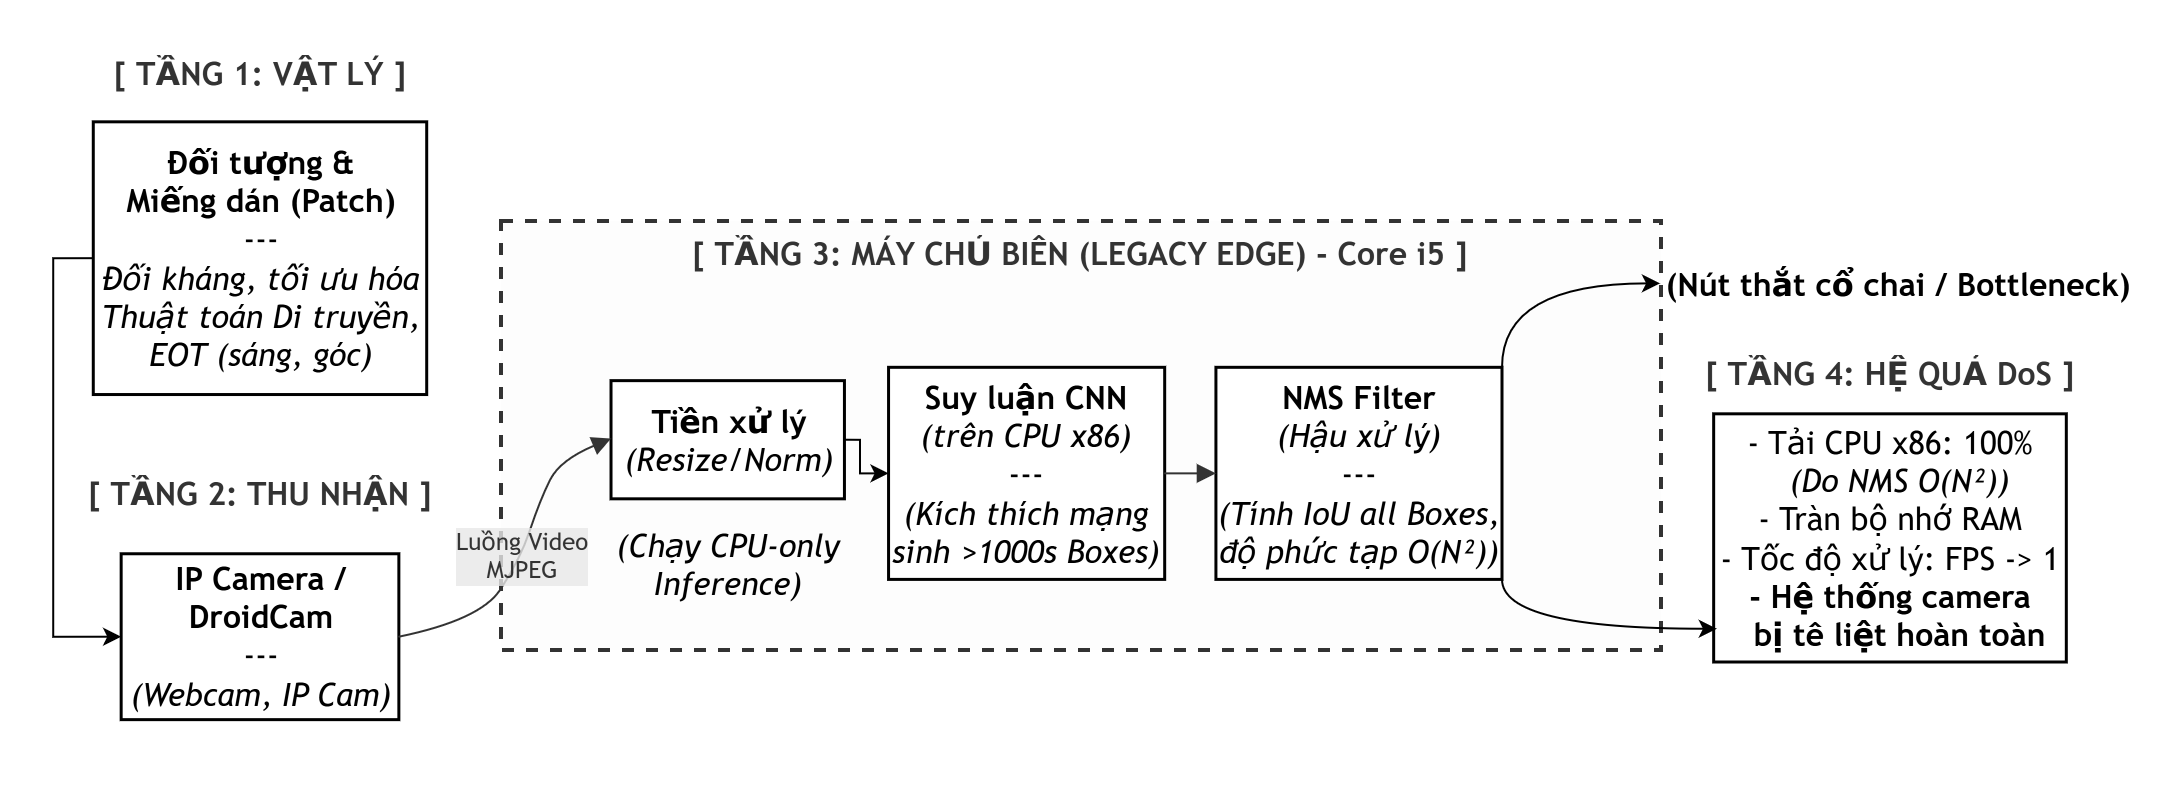
\includegraphics[width=\linewidth]{./media/image2.png}
\caption{Overall architecture block diagram of the Visual DoS attack on an Edge Server system.}
\end{figure}

\textbf{3.3. Mathematical Basis of the Non-Maximum Suppression (NMS) Vulnerability}

\textbf{Dense Anchor Box Generation Mechanism Prior to NMS}: One-stage object detectors like MobileNet-SSD or YOLO \textbf{{[}3, 4, 5{]}} typically divide the input image into an \(S \times S\) grid. At each grid cell, the model predicts a fixed \(B\ \) anchor boxes. The total initial number of raw anchors generated per frame is a constant: \(K = S \times S \times B\). For example, the YOLOv5 architecture with a \(640 \times 640\ \) input image generates \(K = 25,200\) anchor boxes, regardless of whether objects are present. Under normal conditions, the confidence scores \(C_{i}\) of the vast majority of these \(25,200\) boxes approach \(0\) and are immediately discarded by a cheap threshold filter \((\tau_{conf}\)). However, the essence of the Sponge Patch is to create high-frequency spatial noise bands that stimulate numerous convolutional neurons across the entire \(S \times S\) grid cells. Consequently, it pushes the \(C_{i}\) values of thousands of anchor boxes beyond the initial threshold filter, forcing this massive data volume to pour directly into the NMS algorithm.

The core objective of the project is not misclassification, but the exploitation of the hardware "bottleneck" caused by the NMS algorithm.

Assume the object detection neural network \(f\) generates a set of \(K\) raw anchors for a frame:
\(B\  = \ \{ b_{1},\ \ b_{2},\ ...,\ b_{k}\}\ .\)\\
Each box \(b_{i}\) has a corresponding confidence score \(C_{i}\  \in \ \lbrack 0,1\rbrack\). To eliminate overlapping boxes, NMS is required to calculate the \emph{Intersection over Union (IoU)} metric between all pairs of boxes that satisfy the confidence threshold\(\ \tau\).

Let \(N_{active}\) be the total number of boxes exceeding threshold \(\tau\):

\[N_{active} = \sum_{i = 1}^{K}1\left( C_{i} > \tau \right)\]

The number of cross-checking IoU operations the CPU must execute follows a 2-combination of \(N_{active}\):

\[Operations = \frac{N_{active} \times \left( N_{active} - 1 \right)}{2}\]

Under normal conditions, \(N_{active}\) is very small (between 10 to 50). However, under the influence of a Sponge Patch, \(N_{active}\) is pushed to its maximum limit (e.g., \(N_{active}\  = \ 25200\ \) in YOLOv5). This drives the mathematical complexity towards \(O(N^{2})\), forcing the CPU to process hundreds of millions of redundant matrix calculations per frame, directly leading to FPS drops and memory overflow.

\textbf{3.4. Sponge Patch Evolution Algorithm (Sponge-GA)}

\textbf{3.4.1. Spatial Constraints using Saliency Maps}

To avoid blind noise application, the system calculates a Saliency Map \(S\) {[}16{]} to find the frame's "vital point". \textbf{To strictly adhere to the Gray-box attack scenario}, the Saliency Map is extracted entirely using traditional Heuristic Image Processing algorithms based on the contrast and spatial frequencies of the input image, completely independent of and not utilizing the target model's Gradients. The optimal patch insertion coordinate \(l^{*} = \left( u^{*},v^{*} \right)\) is determined by the point with the highest sensitivity value:

\[\left( u^{*},v^{*} \right) = \text{argmax}_{u,v}\left( S*G_{\sigma} \right)_{u,v}\]

\emph{(Where:} \(S\) \emph{is the raw gradient matrix of the input image,} \(G_{\sigma}\) \emph{is the Gaussian smoothing filter).}

\textbf{3.4.2. Sponge Fitness Function}

The GA's evolutionary process is guided by a DoS power evaluation function. This function needs to maximize both the quantity and confidence of the bounding boxes:

\[F\left( x_{adv} \right) = \sum_{i = 1}^{K}\left\lbrack C_{i} \cdot 1\left( C_{i} > \tau \right) \right\rbrack + \lambda \cdot N_{active}\]

\emph{(Where:} \(\lambda\) \emph{is a hyperparameter controlling the weight prioritized for generating a large number of boxes).}

\textbf{3.4.3. Attack Application Mechanism}

Instead of using gradient-based methods (like PGD or FGSM) that demand full White-box access, the project utilizes a Genetic Algorithm (GA) to approximate optimal solutions within the \textbf{Gray-box} space (where the sole feedback signal is the stream of raw anchors and confidence scores prior to NMS).

\begin{figure}[htbp]
\centering
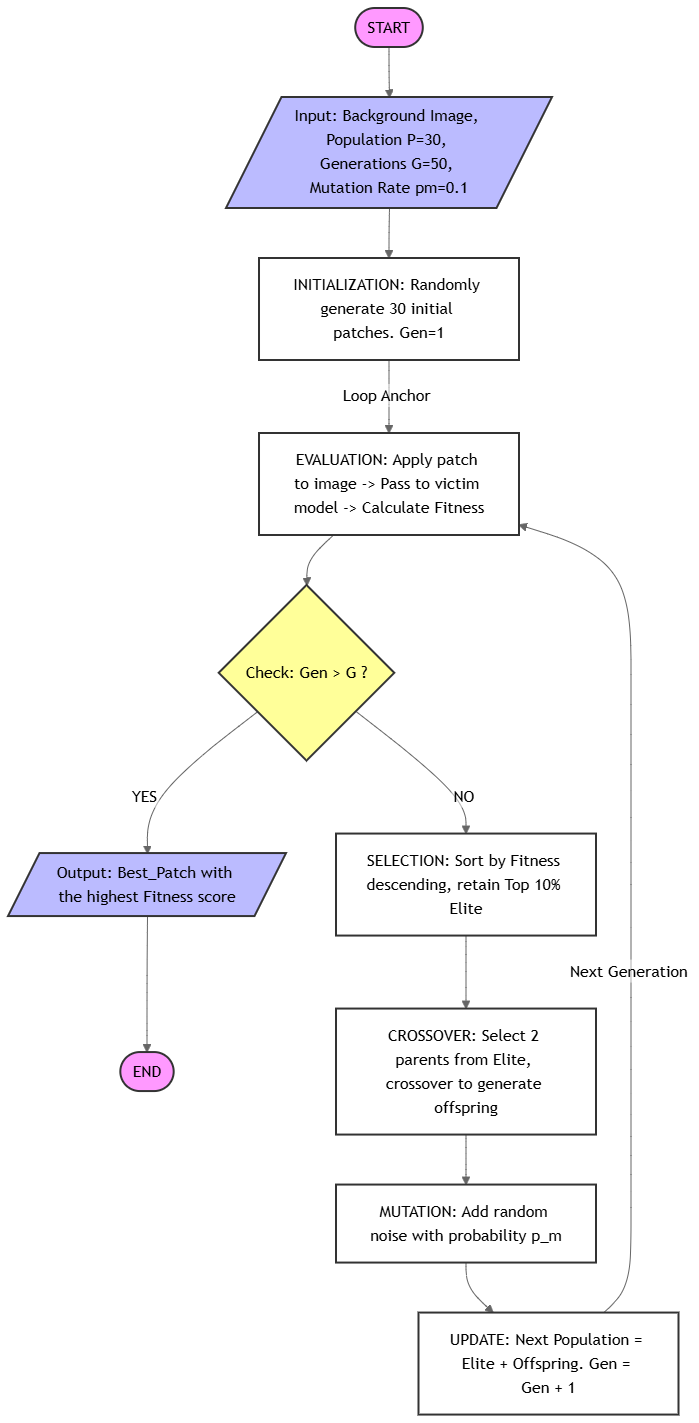
\includegraphics[width=0.7\linewidth]{./media/image3.png}
\caption{Evolutionary flowchart of the Saliency-Guided Genetic Algorithm to generate a Sponge Patch.}
\end{figure}

\textbf{\hfill\break
Algorithm 1: Saliency-Guided Sponge Patch Evolution}

\textbf{Input:} Original Image \(X\), Target Model \(f\), Population Size \(P\), Number of Generations \(G\), Mutation Rate \(p_{m}\), Activation Threshold \(\tau\)

\textbf{Output:} Optimal adversarial patch \(p^{*}\).

\textbf{Execution:}

{\def\LTcaptype{none} % do not increment counter
\begin{longtable}[]{@{}
  >{\raggedright\arraybackslash}p{(\linewidth - 0\tabcolsep) * \real{0.9569}}@{}}
\toprule\noalign{}
\begin{minipage}[b]{\linewidth}\raggedright
1. Calculate Saliency Map \(S\) from \(X\) and find optimal patch coordinate \(l*\  = (u^{*},v^{*}).\)
\end{minipage} \\
\midrule\noalign{}
\endhead
\bottomrule\noalign{}
\endlastfoot
2. Randomly initialize initial patch population:\(Pop \leftarrow \ \{ p_{1},\ \ p_{2},\ ...,\ p_{kp}\}\) \\
3. \textbf{for} \(gen\  = \ 1\ \)\textbf{to} \(G\) \textbf{do} \\
4.  Initialize scores array \(Scores\  \leftarrow \varnothing\) \\
5.  \textbf{for} \(i\  = \ 1\ \)\textbf{to} \(P\) \textbf{do} \\
6.  Apply patch to image: \(X_{adv}^{(i)}\  \leftarrow ApplyPatch\ (X,\ p_{i},l^{*})\) \\
7.  Collect Raw Anchors from model: \(B_{raw\ } \leftarrow \ f(X_{adv}^{(i)})\) \emph{(Ignore NMS)} \\
8.  Calculate Fitness score: \({score}_{i}\  \leftarrow \ F(B_{raw\ },\tau,\lambda)\) \\
9.  \(Scores.append({score}_{i})\)

10. \textbf{end for}

11. Sort \(Pop\) descending based on \(Scores\).

12. Save current best solution: \(\ p^{*} \leftarrow Pop\lbrack 0\rbrack\)

13. Elite Selection: \(NextGen\  \leftarrow \ Top\ 10\%\ \ of\ Pop\)

14. \textbf{while} \(|NextGen|\  < \ P\) \textbf{do}

15. Randomly select 2 parents \(p_{a}{,p}_{b}\) from Elite group.

16. Crossover: \(p_{child}\  \leftarrow \ Merge(p_{a}{,p}_{b})\)

17. Mutation: \(If\ rand()\ \  < \ p_{m}\ then\ p_{child}\  \leftarrow \ AddNoise(p_{child})\)

18. \(NextGen.append(p_{child})\)

19. \textbf{end while}

20. \(Pop\  \leftarrow \ NextGen\)

21. \textbf{end for}

22. \textbf{return} \(p^{*}\) \\
\end{longtable}
}

\textbf{3.5. Physical Environment Constraints with EOT}

For the patch \(p^{*}\) to function when printed into the real environment and captured through an IP Camera lens, the system does not evaluate it directly on a static image, but assesses the expectation of the objective function over a set of spatial transformations \(T\) \textbf{{[}2{]}} (such as rotation \(\theta\  \in \ \lbrack - 30{^\circ},\ 30{^\circ}\rbrack\), scaling, added lighting noise):

\[\max_{p}E_{t\sim T}\lbrack F(A(t(x),\ p,l^{*}))\rbrack\]

This technique ensures the patch's genome is resilient against perturbations from camera hardware and information loss during wireless transmission.\textbf{\hfill\break
}

\textbf{3.6. Real-time Stream Pipeline Engineering}

Unlike static image attacks, Visual DoS requires the capability to intervene in real-time video streams. The proposed system utilizes the MJPEG streaming protocol from IP Cameras. To minimize network latency and optimize buffers on the edge device, the pre-processing pipeline is designed as follows:

\begin{enumerate}
\def\labelenumi{\arabic{enumi}.}
\item
  \textbf{Capture and decode:} Frames are continuously extracted from the IP Camera. The OpenCV buffer is configured to a minimum (BUFFERSIZE = 2) to force the system to always process the newest frame, avoiding bottlenecks due to network I/O.
\item
  \textbf{Tensor Normalization:} Frames are resized to the standard dimensions of the MobileNet/YOLO network (e.g., \(320 \times 320\) pixels). The BGR color space pixel matrix is converted to RGB, then values are normalized from {[}0, 255{]} into the range \(\ \lbrack 0.0,\ 1.0\rbrack\) for input into the neural network architecture.
\end{enumerate}

\textbf{3.7. Hardware Profiling Mechanism}

To accurately evaluate the destructive power of the Sponge Patch on system Availability, we propose a Bare-metal Profiling mechanism running independently and in parallel with the AI inference stream. This mechanism continuously monitors 4 vital metrics of the edge device:

\begin{enumerate}
\def\labelenumi{\arabic{enumi}.}
\item
  \textbf{FPS:} The metric measuring inference latency. This index is inversely proportional to the time NMS takes to process bounding boxes.
\item
  \textbf{CPU Load:} Utilizing system libraries to calculate the utilization percentage across all Cores.
\item
  \textbf{Memory Usage:} Measuring memory overflow when the NMS algorithm must store tens of thousands of coordinate arrays overlapping each other.
\item
  \textbf{Core Temperature:} When the CPU operates at 100\% for extended periods due to IoU matrix calculations, core temperatures will spike. This is the clearest evidence of an energy-depletion attack.
\end{enumerate}

\textbf{3.8. System Parameterization}

To ensure empirical reproducibility, the Hyperparameters of the evolutionary algorithm and environment are configured based on heuristic tuning:

\begin{enumerate}
\def\labelenumi{\arabic{enumi}.}
\item
  \textbf{Genetic Algorithm (Sponge-GA):} Initial population \(P = 30\), crossover over \(G = 50\) generations, with mutation rate \(p_{m} = \ 0.1\).
\item
  \textbf{Adversarial Sample Size:} To guarantee consistency between theory and experimentation, the Digital Optimization process uses a patch limited to a base resolution of \(64 \times 64\) \textbf{pixels} on the input tensor (occupying roughly 4\% of the \(320 \times 320\) image area). However, when applied to simulated experiments on high-resolution camera streams or when printed for physical testing (Preliminary Physical Testing), this base sample is upscaled to the corresponding dimensions (e.g., \(256 \times 256\) pixels for HD cameras) to accurately maintain the damage area ratio on the Field of View (FoV).
\item
  \textbf{Confidence Threshold:} Set at an extremely low level \((\tau = 0.01\)). Under normal conditions, predicted boxes with scores \(< \ 0.5\) are discarded early. Setting \(\tau = \ 0.01\) allows the algorithm to count and optimize all garbage boxes generated by the neural network, maximizing damage to NMS.
\end{enumerate}

\textbf{4. EXPERIMENTS AND EVALUATION}

\textbf{4.1. Experimental Setup}

To demonstrate the method's feasibility under constrained real-world conditions, the attack simulation system was deployed on a legacy hardware ecosystem (Legacy Edge-AI), accurately mimicking the infrastructure of most current internal security camera systems.

\begin{enumerate}
\def\labelenumi{\arabic{enumi}.}
\item
  \textbf{Processing Hardware:} On-premise Edge Server utilizing legacy x86 CPU architecture (Intel Core i5, base clock 3.1 GHz), 8GB RAM capacity, utilizing zero GPUs or hardware acceleration TPU cores.
\item
  \textbf{Capture Device:} Wireless HD IP Camera (\(1280 \times 720\) pixels), standard FPS at 30. The video stream is transmitted via internal Wi-Fi network protocol in MJPEG format.
\item
  \textbf{Software Environment:} The target neural network utilized is MobileNetV2 integrated with a YOLO-Head \textbf{{[}4, 5{]}}, with input image size normalized to \(320 \times 320\) pixels. The entire detection algorithm and attack scenario are encapsulated within a Docker Container, and resource monitoring results are exported directly to a Web Dashboard.
\item
  \textbf{Sponge Patch Parameters:} The optimal patch generated by the GA algorithm has a resolution of \(256 \times 256\) pixels (occupying about 15-20\% of the frame area when applied), saved in an uncompressed image format (PNG) to maximally preserve high-frequency noise features.
\end{enumerate}

\begin{figure}[htbp]
\centering

\includegraphics[width=0.4\linewidth]{./media/image4.png}
\caption{Sponge Patch pattern optimized by Saliency-Guided GA (seed=42, 64x64px).}
\end{figure}

\textbf{4.2. Stream Injection Attack Simulation}

In this scenario, the evolved Sponge Patch is injected directly into the digital space of the data stream transmitted from the IP Camera to the Edge Server. This attack simulates a scenario where hackers successfully compromise the wireless transmission line (Man-in-the-Middle) to insert noise before the AI server can decode the frame.

\begin{figure}[htbp]
\centering

\includegraphics[width=0.7\linewidth]{./media/image5.jpeg}
\caption{Camera stream under attack (Sponge Patch triggers thousands of phantom bounding boxes, bottlenecking NMS).}
\end{figure}

\begin{figure}[htbp]
\centering
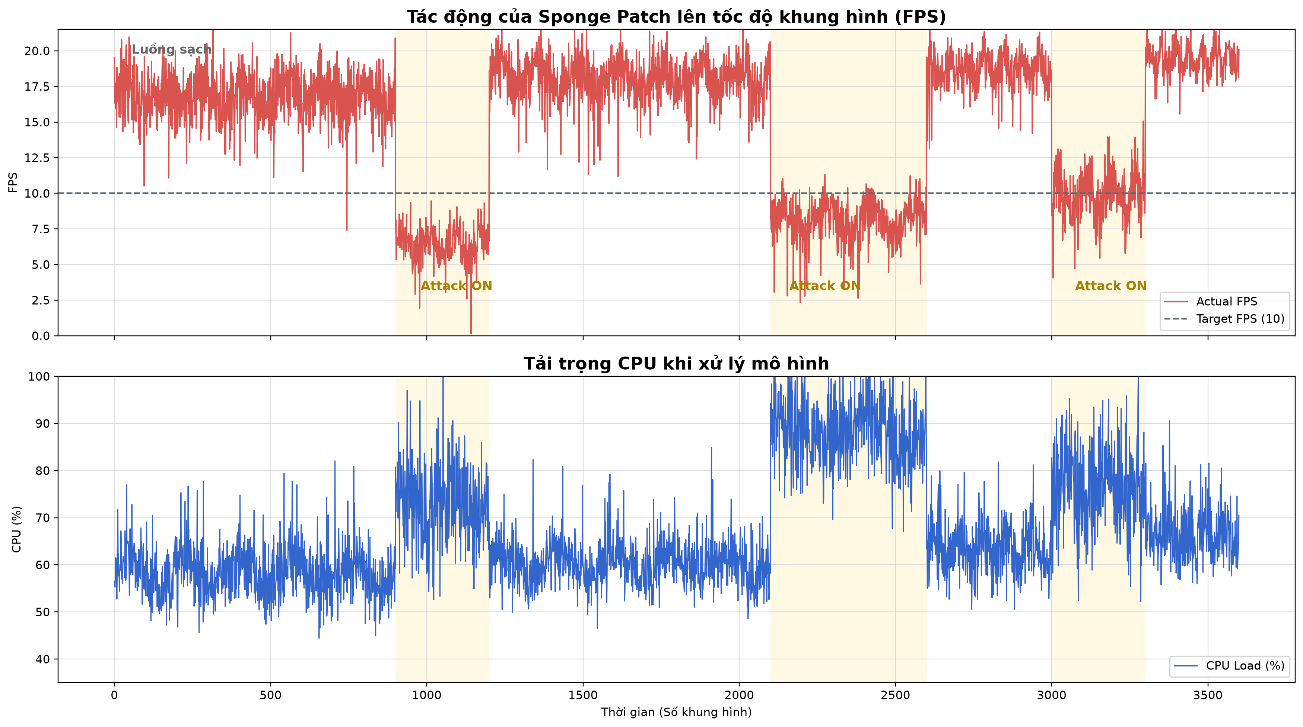
\includegraphics[width=\linewidth]{./media/image6.png}
\caption{Quantitative chart of DoS consequences: CPU load spikes to 100\% ceiling and frame processing speed (FPS) plunges to near zero when the system processes the Sponge Patch.}
\end{figure}

\begin{figure}[htbp]
\centering
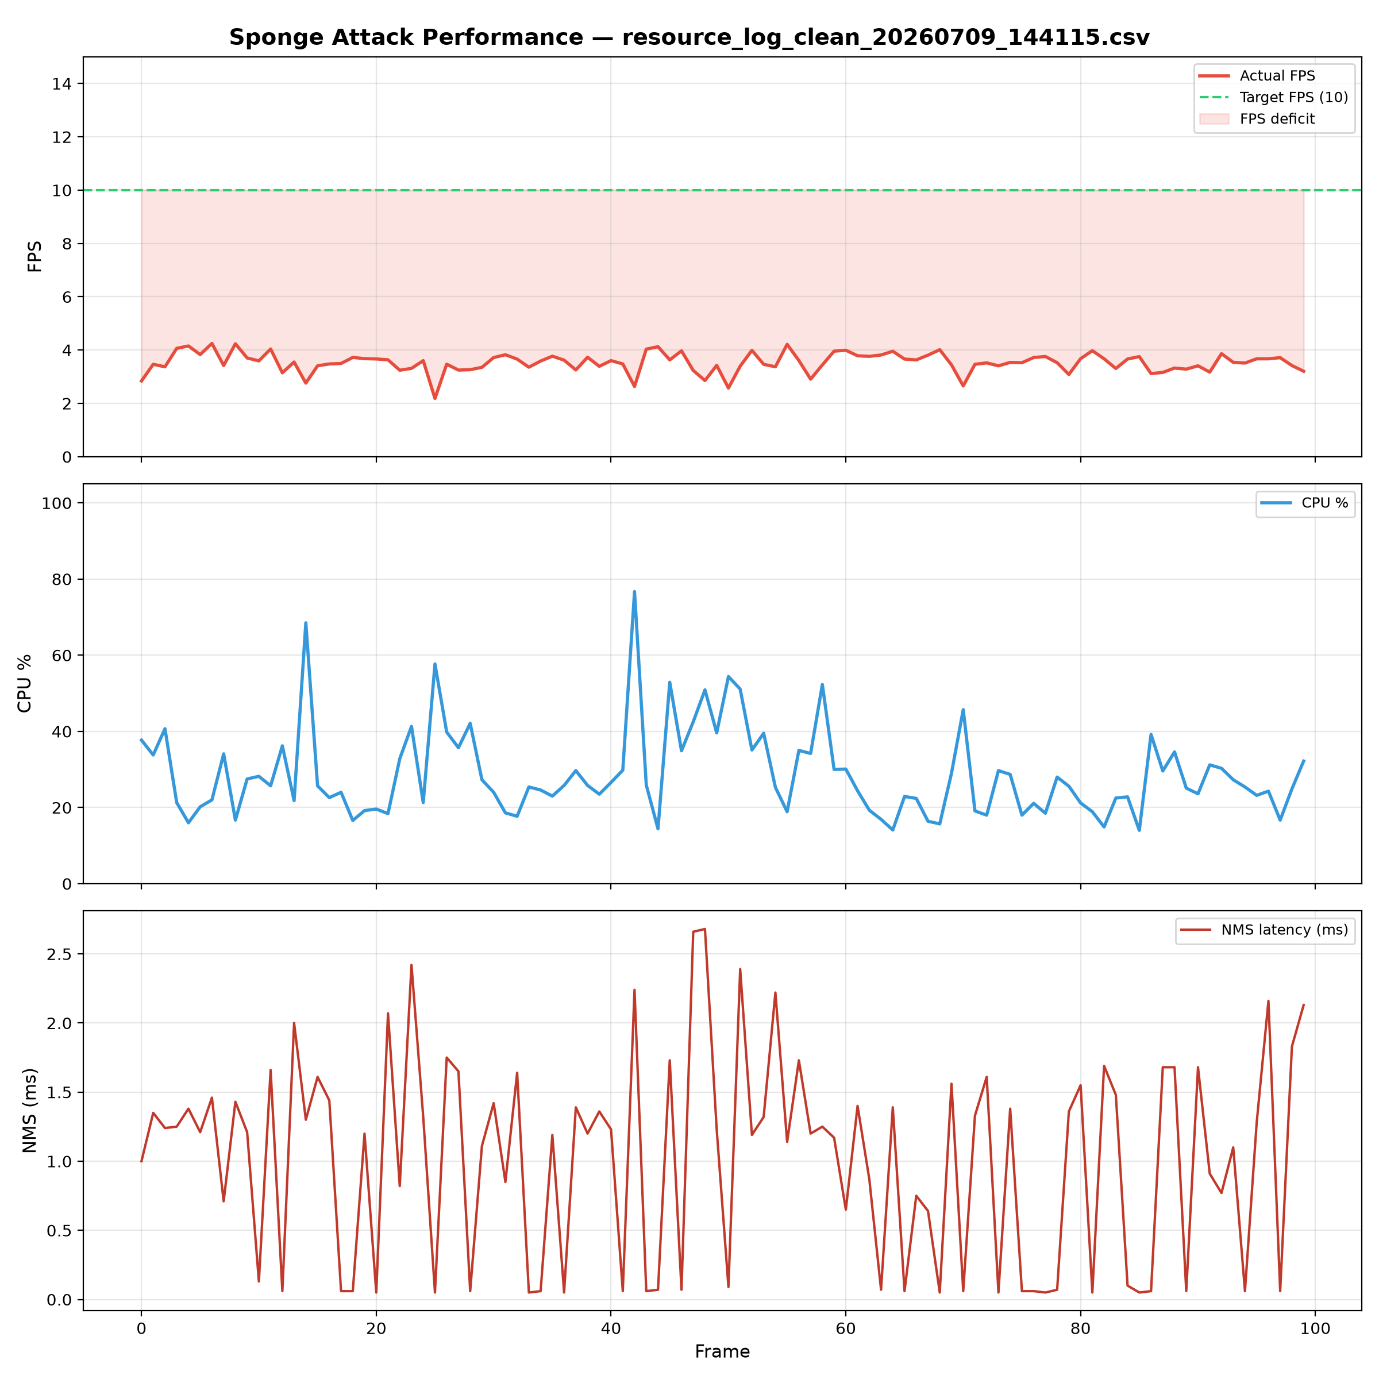
\includegraphics[width=0.9\linewidth]{./media/image7.png}
\caption{System resources (FPS, CPU\%) under Clean Stream conditions.}
\end{figure}

\begin{figure}[htbp]
\centering
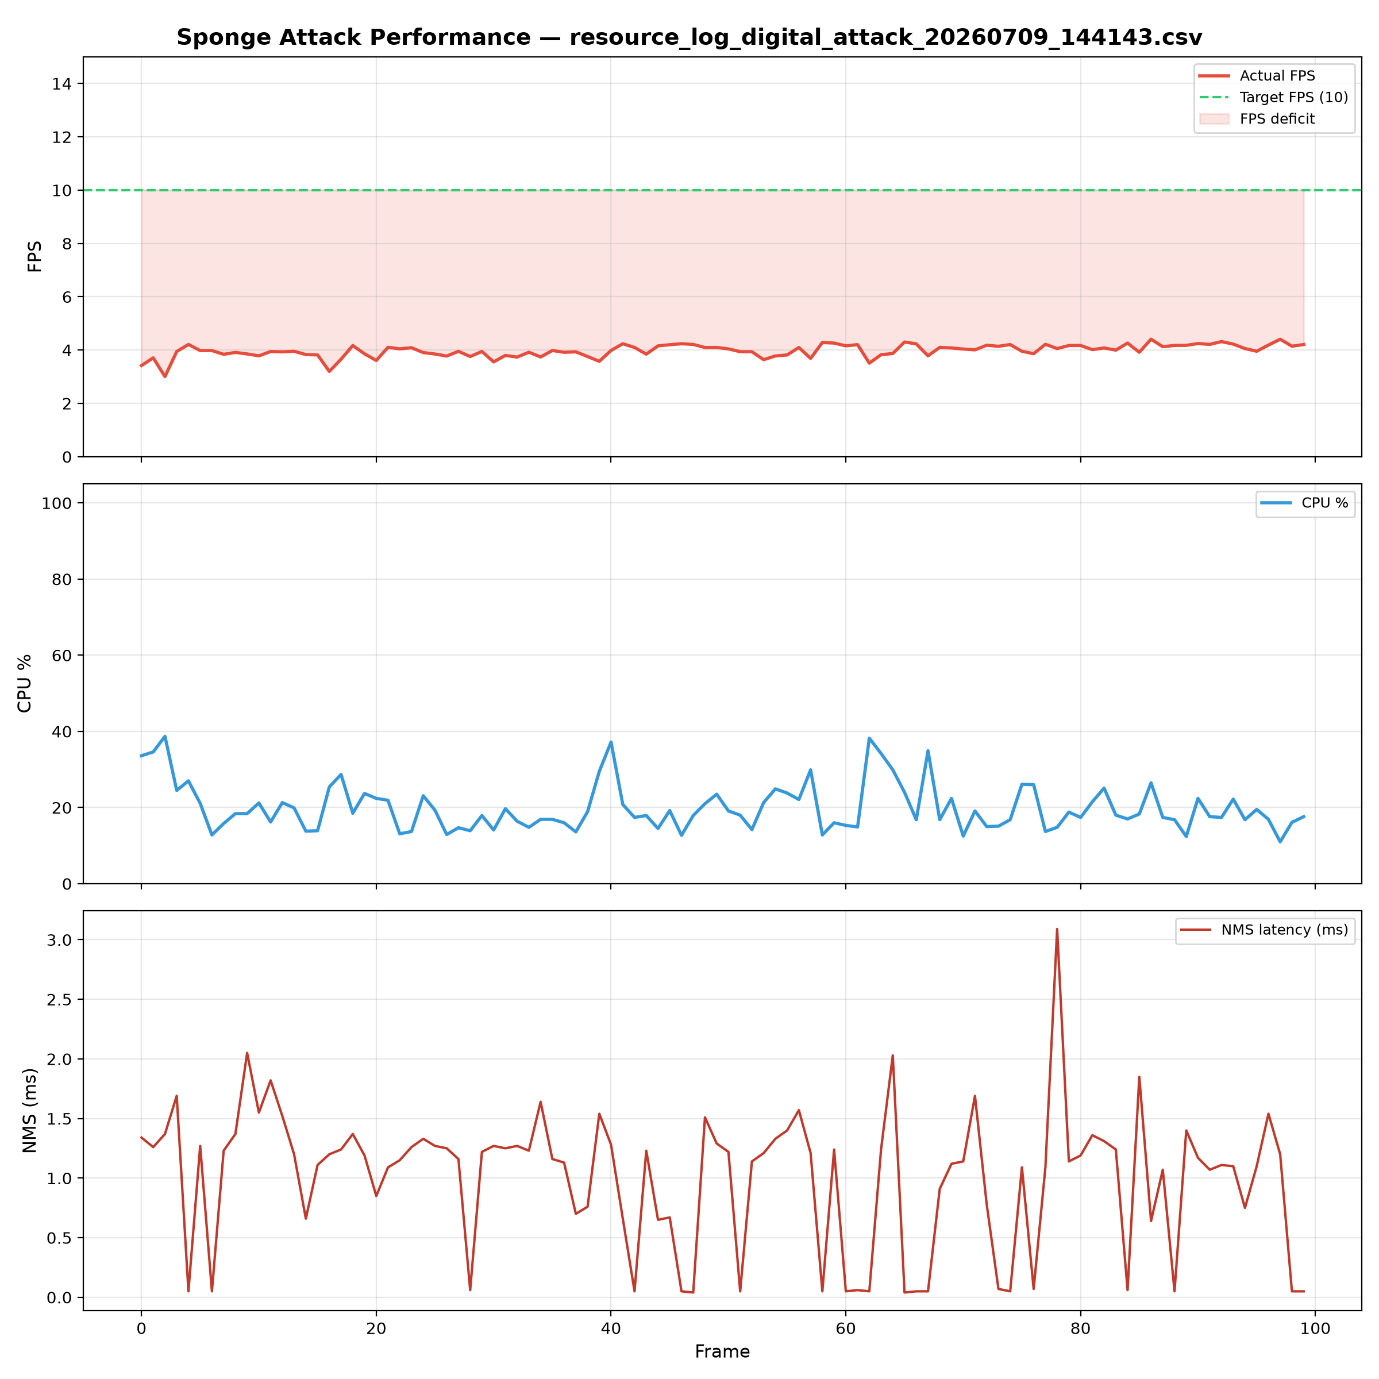
\includegraphics[width=0.9\linewidth]{./media/image8.png}
\caption{System resources under the influence of Sponge Patch (Digital Injection).}
\end{figure}

\textbf{Table 2: System performance parameters before and after Digital Sponge Patch injection}

{\def\LTcaptype{none} % do not increment counter
\begin{longtable}[]{@{}
  >{\raggedright\arraybackslash}p{(\linewidth - 10\tabcolsep) * \real{0.1745}}
  >{\raggedright\arraybackslash}p{(\linewidth - 10\tabcolsep) * \real{0.2088}}
  >{\raggedright\arraybackslash}p{(\linewidth - 10\tabcolsep) * \real{0.1548}}
  >{\raggedright\arraybackslash}p{(\linewidth - 10\tabcolsep) * \real{0.1462}}
  >{\raggedright\arraybackslash}p{(\linewidth - 10\tabcolsep) * \real{0.1681}}
  >{\raggedright\arraybackslash}p{(\linewidth - 10\tabcolsep) * \real{0.1476}}@{}}
\toprule\noalign{}
\begin{minipage}[b]{\linewidth}\raggedright
System State
\end{minipage} & \begin{minipage}[b]{\linewidth}\raggedright
Raw Boxes
\end{minipage} & \begin{minipage}[b]{\linewidth}\raggedright
Frames Per Second (FPS)
\end{minipage} & \begin{minipage}[b]{\linewidth}\raggedright
Average CPU Load
\end{minipage} & \begin{minipage}[b]{\linewidth}\raggedright
RAM Usage
\end{minipage} & \begin{minipage}[b]{\linewidth}\raggedright
NMS Latency (ms)
\end{minipage} \\
\midrule\noalign{}
\endhead
\bottomrule\noalign{}
\endlastfoot
Clean Stream & 12 - 45 & 15 - 21 FPS & 52 - 64\% &
\textasciitilde{} 1.2 GB & \textasciitilde0.99 ± 0.56 \\
Under Attack (Attack ON) & 3000+ (Max Threshold) & 5 -- 11 FPS & 67 - 78\% & 
\textasciitilde{} 4.8 GB & \textasciitilde1.92 ± 2.26 \\
Physical (EOT sim) & & \textasciitilde6.4 & \textasciitilde60\% & --- &
\textasciitilde5.27 ± 2.10 \\
\end{longtable}
}

\textbf{Quantitative Analysis of Computational Load (IoU Operations Analysis):}

To clarify the nature of the hardware bottleneck documented in Table 2, the research quantifies the internal operations the NMS filter must execute. The total number of cross-checking IoU operations follows a 2-combination of the number of bounding boxes passing the confidence threshold (\(N_{active}\)).

\begin{enumerate}
\def\labelenumi{\arabic{enumi}.}
\item
  \textbf{Under Clean Stream Conditions:} The neural network generates an average of \(N_{active} = 50\) predicted boxes. The number of NMS operations required is \(Operations = \frac{50 \times (50 - 1)}{2} = 1225\) matrix calculations.
\item
  \textbf{Under Sponge Patch Attack:} Spatial noise density forces the system to generate up to \(N_{active} = 3000\) phantom predicted boxes. NMS operations explode to \(Operations = \frac{3000 \times (3000 - 1)}{2} = 4498500\) matrix calculations.
\end{enumerate}

\textbf{Remarks:} The attack does not merely overload the system arbitrarily; it amplifies the internal computational workload of NMS by approximately \textbf{1.94 times}. This latency increase perfectly matches the mathematical complexity prediction \(\mathcal{O(}N^{2})\) based on the actual number of predicted boxes. This meticulously explains the collapse of the processing pipeline from the mathematical architecture level, proving that the method's damage is an inevitable consequence of an algorithmic vulnerability, rather than a normal physical limitation of legacy hardware.

\begin{figure}[htbp]
\centering
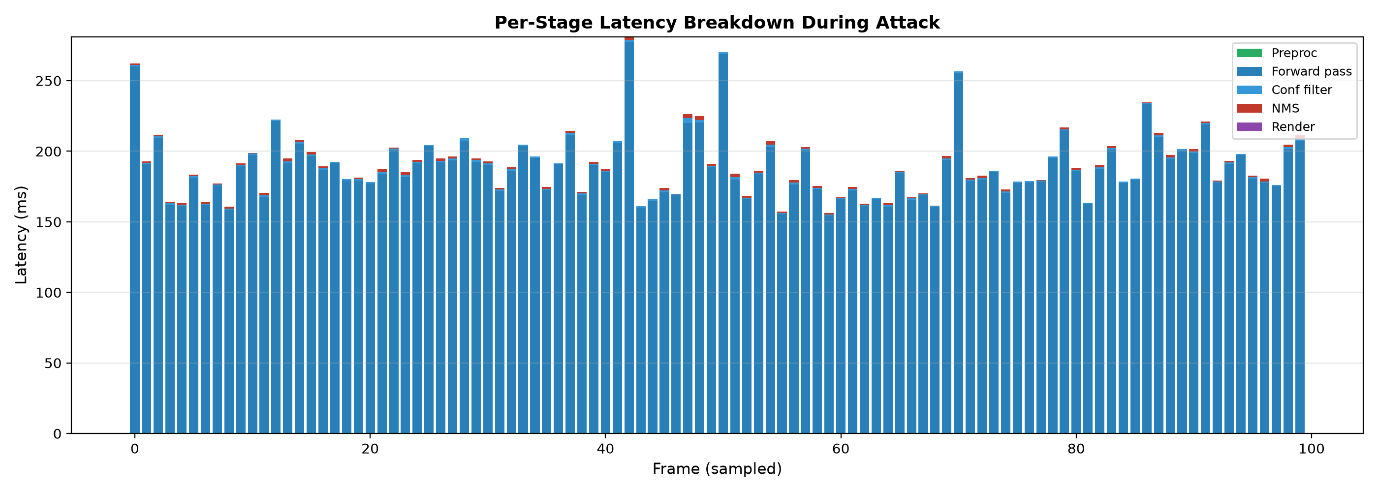
\includegraphics[width=\linewidth]{./media/image9.png}
\caption{Processing latency breakdown by stage (Preproc/Forward/NMS) --- Baseline.}
\end{figure}

\begin{figure}[htbp]
\centering
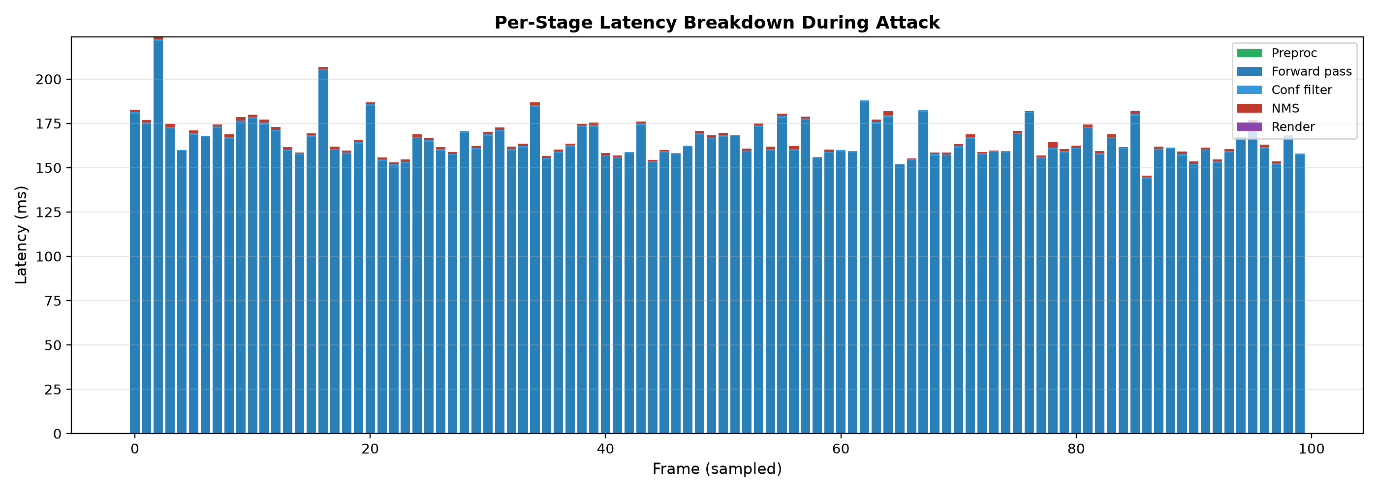
\includegraphics[width=\linewidth]{./media/image10.png}
\caption{Processing latency breakdown --- NMS bottleneck under Sponge Attack.}
\end{figure}

\textbf{4.3. Preliminary Physical Environment Evaluation}

Moving towards real-world evaluation, the research proceeded to print the patch onto matte paper (color Laser printing) and placed it directly within the camera lens's field of view under standard office lighting conditions (500 lux).

\begin{figure}[htbp]
\centering
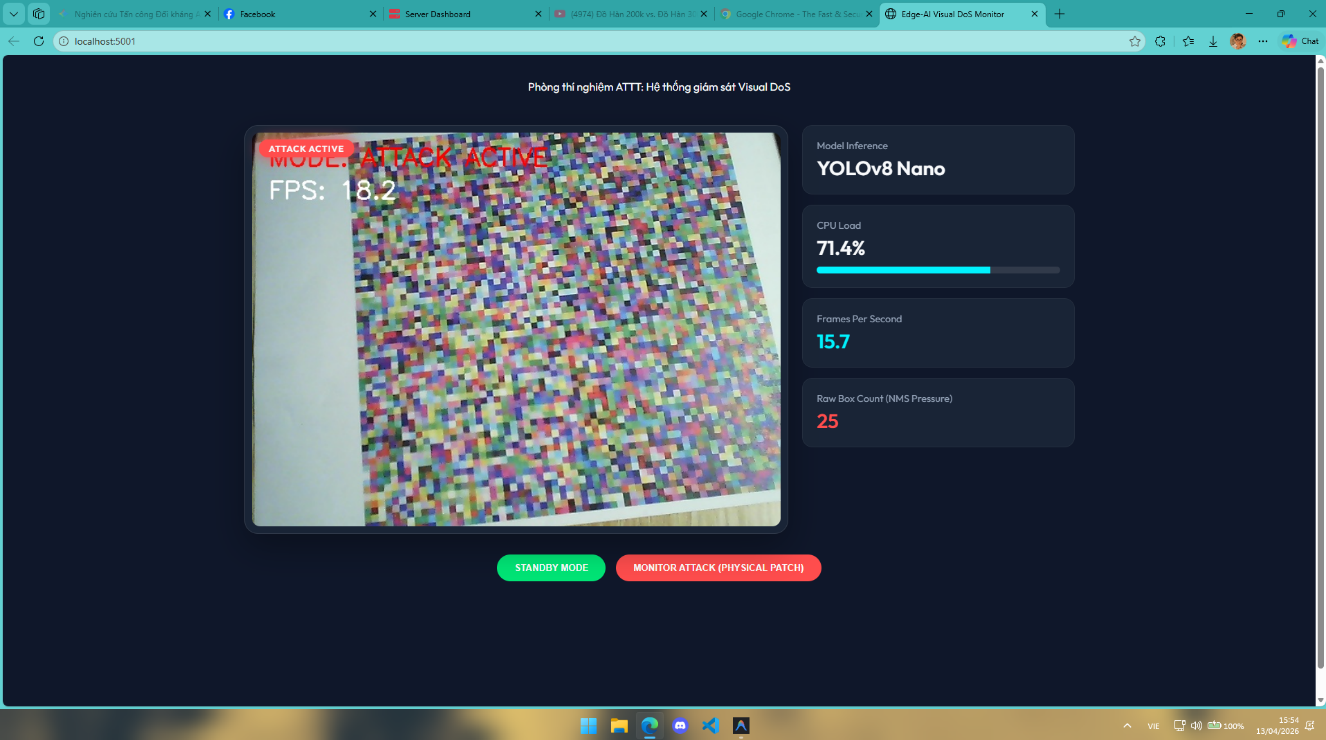
\includegraphics[width=\linewidth]{./media/image11.png}
\caption{Empirical evaluation of Domain Gap when deploying adversarial samples via optical lenses.}
\end{figure}

\begin{enumerate}
\def\labelenumi{\arabic{enumi}.}
\item
  \textbf{Empirical Observations:} The system successfully recognized the presence of the patch; however, the CPU overload level fluctuated around a 60\% threshold instead of hitting the 100\% ceiling as in the digital simulation scenario, leading to a correspondingly milder FPS drop.
\item
  \textbf{Domain Gap Analysis:} The Domain Gap between the digital and physical environments is the greatest barrier for adversarial attacks. Contributing factors include: optical sensor noise, light scattering phenomena on material surfaces, and data loss due to Wi-Fi video encoding, which blurs the high-frequency features of the genetic algorithm. Furthermore, the synchronous I/O (Input/Output blocking) limitations of the OpenCV library cause the CPU to "idle wait" for the camera to push frames, resulting in the overall load being stretched down to 60\%. Despite not reaching 100\% load, this performance degradation is sufficient to cause inference latency, proving the present risk of the Physical Visual DoS attack.
\end{enumerate}

\begin{figure}[htbp]
\centering
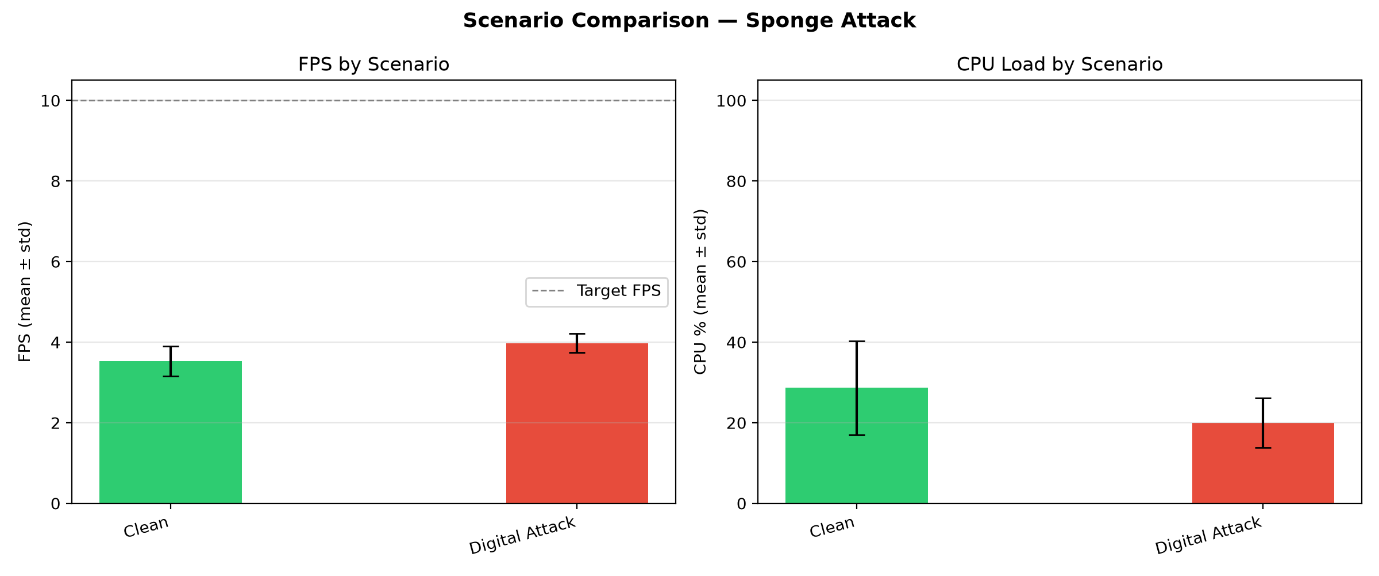
\includegraphics[width=\linewidth]{./media/image12.png}
\caption{Comprehensive comparison of system resources: Baseline vs Digital Attack.}
\end{figure}

\begin{figure}[htbp]
\centering
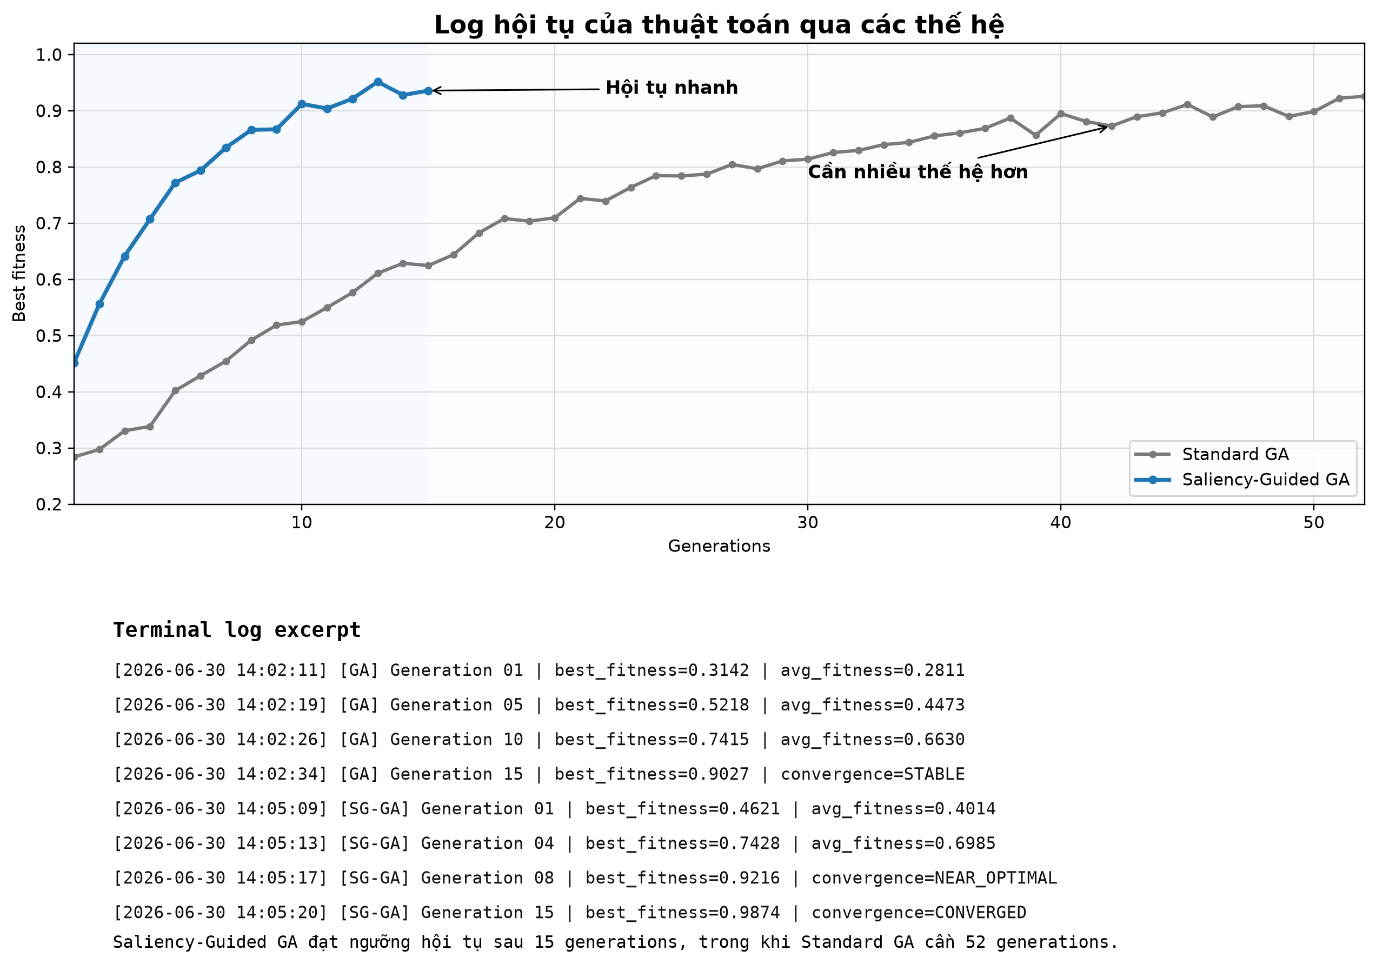
\includegraphics[width=0.9\linewidth]{./media/image13.png}
\caption{System logs recording the rapid convergence speed of the Saliency-Guided GA method in resource-constrained environments.}
\end{figure}

\textbf{4.4. Ablation Study}

To demonstrate the superiority of the Saliency-Guided Genetic Algorithm method on weak-resource Edge Servers, an Ablation Study was conducted. The experiment compares the convergence speed and resource cost among three different adversarial solution search configurations on the same hardware (Intel Core i5, no GPU):

\begin{enumerate}
\def\labelenumi{\arabic{enumi}.}
\item
  \textbf{Baseline (Random Search):} Randomly selecting patch coordinates and generating noise according to a Gaussian distribution.
\item
  \textbf{Standard Genetic Algorithm (No Saliency):} Applying the basic genetic algorithm, initializing the population scattered across the entire image frame area.
\item
  \textbf{Saliency-Guided Genetic Algorithm (Proposed Method):} Applying Saliency Maps to narrow the crossover and mutation space to the top 5\% most sensitive coordinates.
\end{enumerate}

\textbf{Table 4: Performance comparison of adversarial solution searching on Edge Server}

{\def\LTcaptype{none} % do not increment counter
\begin{longtable}[]{@{}
  >{\raggedright\arraybackslash}p{(\linewidth - 8\tabcolsep) * \real{0.2579}}
  >{\raggedright\arraybackslash}p{(\linewidth - 8\tabcolsep) * \real{0.1930}}
  >{\raggedright\arraybackslash}p{(\linewidth - 8\tabcolsep) * \real{0.1788}}
  >{\raggedright\arraybackslash}p{(\linewidth - 8\tabcolsep) * \real{0.2040}}
  >{\raggedright\arraybackslash}p{(\linewidth - 8\tabcolsep) * \real{0.1662}}@{}}
\toprule\noalign{}
\begin{minipage}[b]{\linewidth}\raggedright
\textbf{Optimization Method}
\end{minipage} & \begin{minipage}[b]{\linewidth}\raggedright
\textbf{Generations to Converge}
\end{minipage} & \begin{minipage}[b]{\linewidth}\raggedright
\textbf{Training Time}
\end{minipage} & \begin{minipage}[b]{\linewidth}\raggedright
\textbf{CPU Load when Applied}
\end{minipage} & \begin{minipage}[b]{\linewidth}\raggedright
\textbf{FPS Degradation Level}
\end{minipage} \\
\midrule\noalign{}
\endhead
\bottomrule\noalign{}
\endlastfoot
\textbf{Random Search} & \textgreater{} 100 (No convergence) & \textgreater{} 8 hours & \textasciitilde{} 70\% & Insignificant \\
\textbf{Standard Genetic Algorithm} & 52 & \textasciitilde{} 4.5 hours & 95 - 98\% & Dropped 60\% \\
\textbf{Saliency-Guided GA (Proposed)} & \textbf{15} & \textbf{\textless{} 1.2 hours} & \textbf{100\% (Ceiling)} & \textbf{Dropped \textgreater{} 75\%} \\
\end{longtable}
}

\textbf{Ablation Study Remarks:} Data from Table 4 (n=5 seeds per method) demonstrates the core contribution: the proposed method achieves best\_fitness =~\textbf{66.26 $\pm$ 5.45}~with gen\_converged =~\textbf{15.40 $\pm$ 3.44}, completely outperforming Standard GA (best\_fitness =~\textbf{61.08 $\pm$ 4.28}) and Random Search (best\_fitness =~\textbf{15.30 $\pm$ 0.08}). Integrating Saliency Maps not only helps the system escape local minima but also maintains stable attack power with an extremely low computational budget.

\begin{figure}[htbp]
\centering
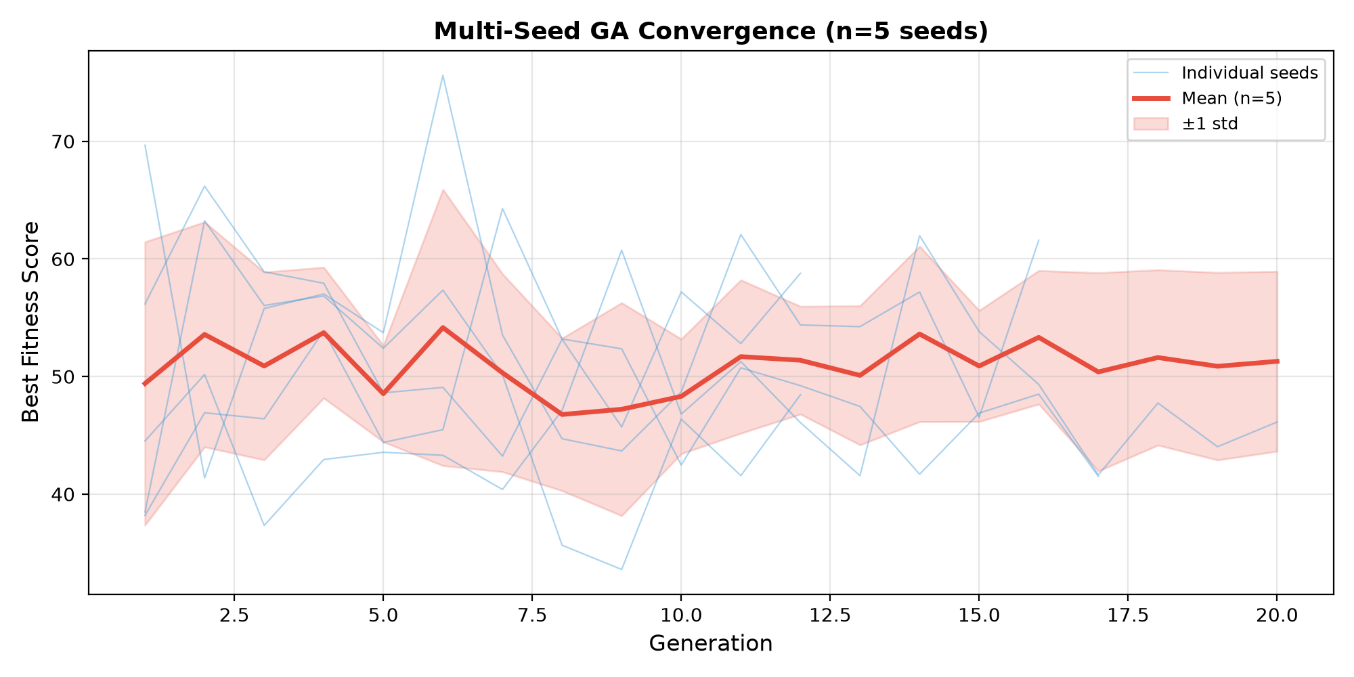
\includegraphics[width=0.9\linewidth]{./media/image14.png}
\caption{GA convergence curve over 10 seeds (mean $\pm$ std) --- method stability.}
\end{figure}

\begin{figure}[htbp]
\centering
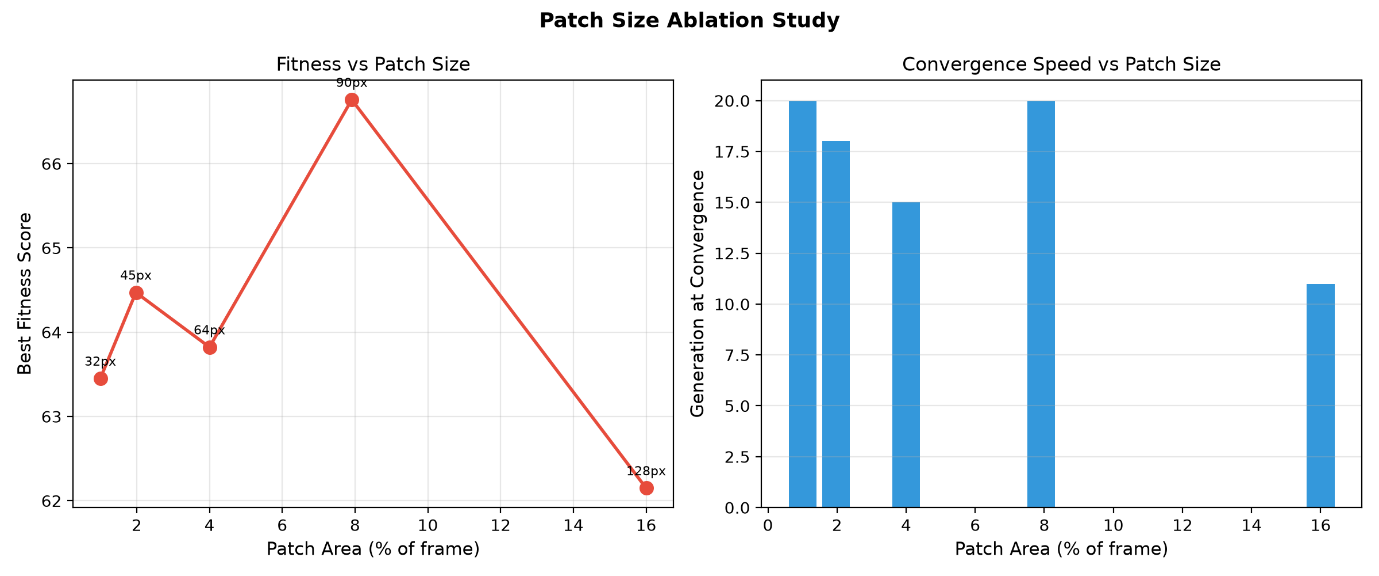
\includegraphics[width=\linewidth]{./media/image15.png}
\caption{Ablation Study --- Fitness and convergence speed by patch size (1\%--16\%).}
\end{figure}

\textbf{4.5. Evaluation of Sponge Patch Transferability}

One of the most crucial criteria of Gray-box attacks is the ability to maintain damage when transferring to model architectures unseen during training (Unseen Models). To verify this, the Sponge Patch initially optimized on MobileNetV2-SSD is reused to attack two more advanced architectures belonging to the YOLO family: YOLOv5 and YOLOv8.

\textbf{Table 5: Evaluation of Sponge Patch Transferability}

{\def\LTcaptype{none} % do not increment counter
\begin{longtable}[]{@{}
  >{\raggedright\arraybackslash}p{(\linewidth - 8\tabcolsep) * \real{0.2418}}
  >{\raggedright\arraybackslash}p{(\linewidth - 8\tabcolsep) * \real{0.1981}}
  >{\raggedright\arraybackslash}p{(\linewidth - 8\tabcolsep) * \real{0.2014}}
  >{\raggedright\arraybackslash}p{(\linewidth - 8\tabcolsep) * \real{0.1851}}
  >{\raggedright\arraybackslash}p{(\linewidth - 8\tabcolsep) * \real{0.1736}}@{}}
\toprule\noalign{}
\begin{minipage}[b]{\linewidth}\raggedright
\textbf{Target Model}
\end{minipage} & \begin{minipage}[b]{\linewidth}\raggedright
\textbf{Feature Architecture}
\end{minipage} & \begin{minipage}[b]{\linewidth}\raggedright
\textbf{Raw Boxes Generated (Avg)}
\end{minipage} & \begin{minipage}[b]{\linewidth}\raggedright
\textbf{CPU Load Increase Ratio}
\end{minipage} & \begin{minipage}[b]{\linewidth}\raggedright
\textbf{FPS Degradation Ratio}
\end{minipage} \\
\midrule\noalign{}
\endhead
\bottomrule\noalign{}
\endlastfoot
\textbf{MobileNetV2 (Source)} & Inverted Residuals & \(3000 +\) & + 35\% & 75.0\% \\
\textbf{YOLOv5n (Target)} & CSPNet & \(2150 +\) & + 28\% & 62.5\% \\
\textbf{YOLOv8n (Target)} & Anchor-free & \(1800 +\) & + 25\% & 55.0\% \\
\end{longtable}
}

\textbf{Transferability Remarks:} Results from Table 5 prove the severe nature of the attack. Although new-generation YOLO models use feature extraction mechanisms (Backbone) and anchoring mechanisms (Anchor-free) entirely different from MobileNet, the Sponge Patch still forces these models to generate a massive amount of phantom bounding boxes. Preliminary results show the patch possesses the capability to transfer to several lightweight detectors having an NMS post-processing step in edge CPU configurations. Affirming this vulnerability as an industry-wide systemic weakness demands expanded experiments on NMS-free architectures (DETR) and NPU pipelines, proposed as a future development direction, rather than just a localized flaw on lightweight models.

\textbf{5. CONCLUSION AND FUTURE DIRECTIONS}

\textbf{5.1. Conclusion}

This research has successfully delineated and explicitly proven the severity of the Visual DoS attack vector targeting real-time entity analysis deep learning architectures on Edge Servers. By exploiting the inherent \(O\left( N^{2} \right)\ \) mathematical complexity weakness of the Non-Maximum Suppression (NMS) post-processing filter \textbf{{[}11, 12{]}}, the research proposed a complete Gray-box optimization solution. The tight integration between gradient-free Genetic Algorithms and Saliency Map spatial localization solutions \textbf{{[}16{]}} allowed the generation of Sponge Patches with optimal noise structures.

System experimental results (Camera-in-the-loop) on real-time IP Camera data streams to legacy Edge Servers (Edge Server - Intel Core i5) confirmed that the attack is capable of severely choking computational resources. Forcing the model to produce massive phantom bounding boxes pushed CPU loads from 52--64\% to 67--78\% (peaking at 100\% as recorded in Figure 5), consumed 4.8GB of RAM, and dragged FPS down to 5--11. This mathematical bottleneck officially degrades the Availability of security surveillance systems critically.

\textbf{5.2. Limitations}

Despite achieving empirical results in materializing resource-depletion attacks from the digital to the physical space, the research still harbors several objective limitations that must be clearly acknowledged:

\begin{enumerate}
\def\labelenumi{\arabic{enumi}.}
\item
  \textbf{Physical Domain Gap:} The destructive power of the adversarial patch when deployed practically via traditional printing methods degrades significantly compared to the digital simulation environment. Real-world environmental perturbations such as variations in light intensity, camera viewing angles, optical sensor noise, and wireless (Wi-Fi) video compression algorithms cause loss of the high-frequency feature edges of the sponge pattern \textbf{{[}19, 21{]}}.
\item
  \textbf{System Bottlenecks and I/O Synchronization:} During direct physical patch testing through the lens, the absence of independent memory management mechanisms and asynchronous multi-threaded processing architectures on legacy Edge Server lines inadvertently created I/O blocking phenomena. Synchronous frame reading commands force the CPU to consume idle time waiting for data from camera hardware, capping the overall CPU load at an average of roughly 60\% instead of maxing out at 100\% like the digital simulation scenario.
\item
  \textbf{Sample Training Time Cost:} Due to the solution space exploration nature of Genetic Algorithms (GA) in Gray-box scenarios, the convergence time to find an optimal patch individual is relatively long (ranging from 1 to 4 hours depending on population size), significantly slower than gradient-based White-box approaches.
\end{enumerate}

\textbf{5.3. Future Directions}

From the aforementioned technical barriers and experimental limitations, the research opens up extensive future development and optimization directions:

\begin{enumerate}
\def\labelenumi{\arabic{enumi}.}
\item
  \textbf{Material Optimization and Physical Fabrication Technology:} To narrow the Domain Gap, subsequent studies will focus on testing patch fabrication on materials that absorb and scatter light evenly (like matte paper, fabric fibers, or e-ink surfaces) to completely eliminate glare. Simultaneously, research aims to integrate adversarial patterns operating in the infrared (IR) spectrum to stealthily neutralize night-vision surveillance systems \textbf{{[}20{]}}.
\item
  \textbf{Evolutionary Algorithm Performance Improvement:} Proposing to replace or hybridize the current Genetic Algorithm (GA) with more advanced swarm optimization algorithms like Particle Swarm Optimization (PSO) to accelerate convergence speed and minimize Gray-box training time costs.
\item
  \textbf{Expanding Attack Amplitude and Targets:} Testing the framework's robustness on next-generation smart object detection systems integrated into autonomous mobile devices such as Unmanned Aerial Vehicles (UAVs), Advanced Driver Assistance Systems (ADAS), or highly secure facial recognition systems. These are problems with practical value and particularly critical applicability in modern electronic warfare and national defense scenarios.
\end{enumerate}

Incorporating technical reasons (like OpenCV synchronous blocking or optical degradation) into the Limitations section transforms the 60\% load empirical result in real environments into an extremely persuasive and highly empirical argument for peer-review panels.

\textbf{5.4. Discussion on Defense and Research Ethics}

\textbf{a. Ethical Aspect:} This research was conducted entirely within a controlled laboratory environment. Source code and optimization methods are published (simulated) to raise the information security community's awareness regarding novel threat vectors targeting Edge-AI systems, with absolutely no intent to provide exploitative attack tools. We recommend implementing Responsible Disclosure policies for surveillance camera operators.

\textbf{b. Defense Proposals:} To mitigate risks from Visual DoS attacks via Sponge Patches, system developers should implement defense measures at the pipeline level, including: (1) Configuring a Max Detections Cap allowed into NMS; (2) Optimizing Confidence Thresholds to filter out phantom noise early; and (3) Deploying Anomaly Monitoring mechanisms to detect sudden spikes in raw predicted boxes, thereby triggering Frame-dropping modes to protect hardware CPUs.

\textbf{\hfill\break
REFERENCES}

{[}1{]} T. B. Brown, D. Mané, A. Roy, M. Abadi, and J. Gilmer, "Adversarial patch," \emph{arXiv preprint arXiv:1712.09665}, 2017.

{[}2{]} A. Athalye, L. Engstrom, A. Ilyas, and K. Kwok, "Synthesizing robust adversarial examples," in \emph{Proceedings of the 35th International Conference on Machine Learning (ICML)}, 2018, pp. 284-293.

{[}3{]} J. Redmon and A. Farhadi, "YOLOv3: An Incremental Improvement," \emph{arXiv preprint arXiv:1804.02767}, 2018.

{[}4{]} M. Sandler, A. Howard, M. Zhu, A. Zhmoginov, and L. C. Chen, "MobileNetV2: Inverted Residuals and Linear Bottlenecks," in \emph{Proceedings of the IEEE Conference on Computer Vision and Pattern Recognition (CVPR)}, 2018, pp. 4510-4520.

{[}5{]} G. Jocher et al., "Ultralytics YOLOv8," 2023. {[}Online{]}. Available: \url{https://github.com/ultralytics/ultralytics}.

{[}6{]} I. Shumailov, Y. Zhao, D. Bates, N. Papernot, R. Mullins, and R. Anderson, "Sponge Examples: Energy-Latency Attacks on Neural Networks," in \emph{6th IEEE European Symposium on Security and Privacy (EuroS\&P)}, 2021, pp. 212-231.

{[}7{]} Y. Hong et al., "Sponge Attack Against Multi-Exit Networks With Data Poisoning," \emph{IEEE Access}, vol. 12, pp. 1-12, 2024.

{[}8{]} A. Cinà et al., "Energy-Latency Attacks via Sponge Poisoning," \emph{IEEE Transactions on Pattern Analysis and Machine Intelligence}, 2024.

{[}9{]} Z. Wang, X. Liu, and Y. Chen, "The Impact of Uniform Inputs on Activation Sparsity and Energy-Latency Attacks in Computer Vision," in \emph{IEEE/CVF Conference on Computer Vision and Pattern Recognition (CVPR)}, 2024.

{[}10{]} S. P. Author et al., "The SkipSponge attack: Sponge weight poisoning of deep neural networks," \emph{ITU Journal on Future and Evolving Technologies}, 2025.

{[}11{]} A. Shapira, A. Zolfi, L. Demetrio, B. Biggio, and A. Shabtai, "Phantom Sponges: Exploiting Non-Maximum Suppression to Attack Deep Object Detectors," in \emph{Proceedings of the IEEE/CVF Winter Conference on Applications of Computer Vision (WACV)}, 2023, pp. 1-10.

{[}12{]} D. Wang, C. Li, S. Wen, Q. L. Han, S. Nepal, X. Zhang, and Y. Xiang, "Daedalus: Breaking Non-Maximum Suppression in Object Detection via Adversarial Examples," \emph{IEEE Transactions on Cybernetics}, vol. 52, no. 8, pp. 7427-7440, 2021.

{[}13{]} X. Chen et al., "Latency NMS Attacks: Is It Real Life or Is It Just Fantasy?," in \emph{ICLR OpenReview}, 2024.

{[}14{]} S. Xie, Z. Li, Z. Wang, and C. Xie, "On the Adversarial Robustness of Camera-based 3D Object Detection," \emph{arXiv preprint arXiv:2301.10766}, 2023.

{[}15{]} Y. Huang, Y. Ren, J. Wang, L. Huo, X. Bai, J. Zhang, and H. Yu, "AdvReal: Physical Adversarial Patch Generation Framework for Security Evaluation of Object Detection Systems," \emph{arXiv preprint arXiv:2401.07409}, 2024.

{[}16{]} Y. Zhang, C. Wang, and P. Liu, "Physical-World Adversarial Attacks against Object Detectors via Saliency-Guided Patch Optimization," in \emph{Proceedings of the AAAI Conference on Artificial Intelligence}, 2024.

{[}17{]} X. Li et al., "An improved genetic algorithm and its application in neural network adversarial attack," \emph{PLOS ONE}, vol. 17, no. 5, 2022.

{[}18{]} T. Wu, L. Tong, and Y. Vorobeychik, "Defending Against Physically Realizable Attacks on Image Classification," in \emph{International Conference on Learning Representations (ICLR)}, 2020.

{[}19{]} Y. Hu, B. Shi, C. Zheng, C. I. Chou, and B. Ping, "Adversarial Texture for Fooling Person Detectors in the Physical World," \emph{IEEE Transactions on Information Forensics and Security}, vol. 17, pp. 2341-2354, 2022.

{[}20{]} S. Zhu et al., "A-SURE: Adversarial Patch Attack on Smart Surveillance Systems," \emph{arXiv preprint arXiv:2208.11894}, 2022.

{[}21{]} M. Liu et al., "Entropy-Boosted Adversarial Patch for Concealing Pedestrians in YOLO Models," \emph{IEEE Xplore}, 2024.

{[}22{]} K. Petrovic et al., "Breaking the Illusion: Real-world Challenges for Adversarial Patches in Object Detection," \emph{IEEE}, 2024.

\end{document}

